\apendice{Documentación técnica de programación}

\section{Introducción}
En este anexo se muestra toda la información necesaria para que un desarrollador pueda poner en funcionamiento el \textit{software} de este proyecto.
Además, se da una explicación sobre la estructura del código y aquellos aspectos que puedan ser importantes para cualquier desarrollador que vea por primera vez el código desarrollado.

\section{Estructura de directorios}
La estructura de los directorios del proyecto es la siguiente:
\begin{itemize}
\item \textbf{docs:} Contiene la documentación del proyecto.
\item \textbf{src:} Dentro de este directorio se encuentra el código fuente del proyecto desarrollado.
\end{itemize}

Este anexo va a centrarse en la explicación del contenido del directorio \texttt{src}.
En la figura~\ref{fig:directorios} se puede ver la distribución de los directorios que se encuentran dentro de \texttt{src}.

\begin{figure}
	\centering
	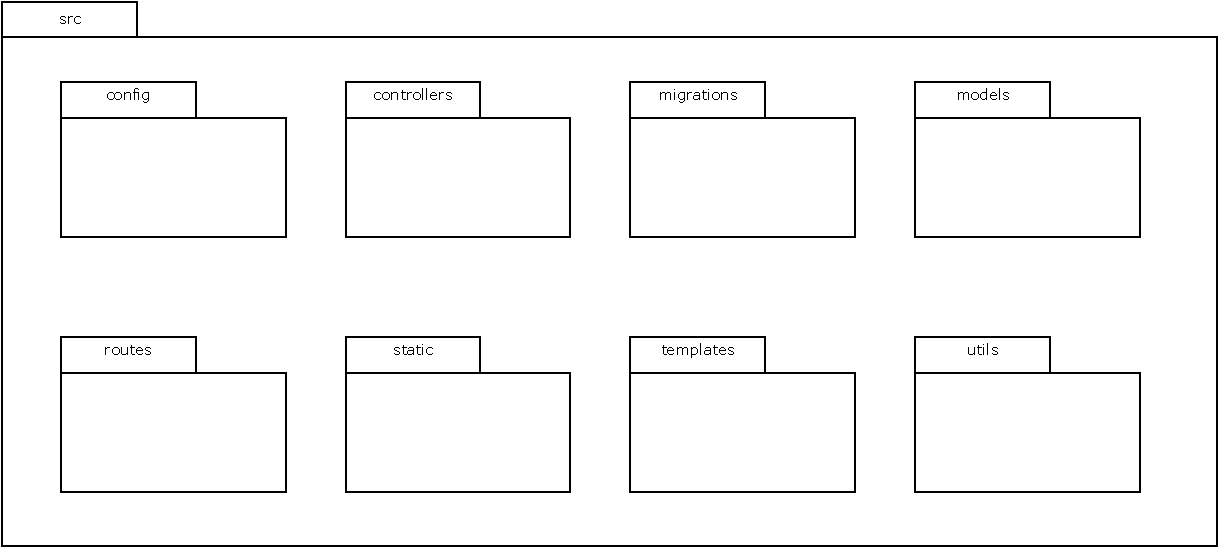
\includegraphics[width=\textwidth]{../img/Anexos/directorios.pdf}
	\caption{\textit{Directorios del proyecto}}\label{fig:directorios}
\end{figure}

A continuación se da una explicación de lo contenido en cada directorio:
\begin{itemize}
\item \texttt{src:} 
Es el directorio principal del código fuente del proyecto que contiene a todos los demás. 
Además, en su interior se encuentra el fichero \texttt{app.py} desde el que se carga la configuración y se arranca la aplicación, el fichero \texttt{forms.py} que contiene todos los formularios generados a partir de al biblioteca WTForms y el fichero \texttt{decorators.py} que contiene aquellas funciones encargadas de detectar los permisos del usuario activo y su \textit{token}.
Por otro lado, también se encuentran los ficheros \texttt{Procfile} necesario para desplegar la aplicación en Heroku, \texttt{requirements.txt} que contiene todas las bibliotecas junto a su versión requerida y el fichero \texttt{runtime.txt} también necesario para desplegar en Heroku donde se indica la versión de Python.

\item \texttt{config:} 
Contiene tres ficheros necesarios para la configuración del proyecto.
El fichero \texttt{config.py} indica la configuración general del proyecto mientras que los ficheros \texttt{development.py} y \texttt{production.py} contienen la configuración necesaria para el despliegue en modo desarrollo y modo producción respectivamente.

\item \texttt{controllers:}
En este directorio se encuentran todos los controladores del proyecto.

\item \texttt{migrations:}
Es un directorio perteneciente a la librería Flask-Migrate. 
Este directorio es utilizado para almacenar la configuración de la biblioteca y las diferentes migraciones creadas para actualizar la base de datos evitando la pérdida de información almacenada. (En principio, no sería necesario tocar nada de este directorio).

\item \texttt{models:}
Aquí se encuentran todos los ficheros respectivos a los modelos de la aplicación web. Es decir, aquellos objetos que se crean y almacenan en la aplicación.
Desde cada uno de estos ficheros también se define la estructura de sus tablas en la base de datos.

\item \texttt{routes:}
Este directorio almacena los diferentes ficheros que definen las rutas de la aplicación, organizadas por \textit{blueprints}.

En estos ficheros se indican los decoradores de cada ruta y la acción del controlador asociada que se debe ejecutar con la petición a esa ruta. 
Además, se define el tipo de petición HTTP permitida por ruta.

\item \texttt{static:} 
Como su nombre indica, este directorio contiene todos aquellos ficheros estáticos de la aplicación que van a ser cargados por las vistas. 
Los ficheros que contiene son accesibles desde un navegador y aquí se almacenan imágenes, ficheros CSS, ficheros de JavaScript y las librerías de JavaScript cargadas desde el sistema de gestión de paquetes NPM, junto al fichero de configuración donde se indican las bibliotecas y su versión llamado \texttt{package.json}.

\item \texttt{templates:}
Este directorio agrupa todas aquellas vistas de la aplicación web.
Dentro se encuentra dividido a su vez por otros directorios con el nombre de los diferentes modelos para tener más organizadas las vistas.

En este directorio también se encuentra el fichero \texttt{base\_template.html} que define la plantilla base de todas las demás vistas.
Desde este fichero se define la carga de los ficheros CSS y \textit{scripts} de JavaScript, además de otros elementos como el menú de la aplicación.

En este fichero todos los elementos se encuentran divididos por bloques para cargar solo aquellos necesarios.
Por ejemplo, el footer solo se carga en la vista de \textit{login}, pero el bloque de carga se define aquí.

\item \texttt{utils:}
Este directorio está creado para mejorar la carga y organización de la aplicación.
Dentro del directorio se encuentra el fichero \texttt{db.py} donde se cargan las bibliotecas relativas a la base de datos como SQLAlchemy o Flask-Migrate.
\end{itemize}

\section{Manual del programador}
En esta sección se pretenden explicar algunos detalles necesarios para el entendimiento del código desarrollado teniendo en cuenta la explicación de la estructura de directorios dada en la sección anterior.



\section{Compilación, instalación y ejecución del proyecto}

\section{Pruebas del sistema}
